\documentclass[conference]{IEEEtran}
\IEEEoverridecommandlockouts

\usepackage{amsmath}
\usepackage{newtxtext,newtxmath}
\usepackage{graphicx}
\usepackage{booktabs}
\usepackage{siunitx}
\usepackage[hidelinks]{hyperref}
\usepackage{cite}

\graphicspath{{figures/}}
\newcommand{\Cz}{C0}
\newcommand{\Co}{C1}
\newcommand{\Ct}{C2}
\newcommand{\Cr}{C3}

\begin{document}

\title{Physics, Learning, or Both?\\ Correcting a Sampling-Based MPC after an Unknown Payload Change}

\author{\IEEEauthorblockN{Shengwei Li}
\IEEEauthorblockA{The University of Sydney, NSW, Australia\\
Project technical report, October 2026}}

\maketitle

\begin{abstract}
A robot arm that picks up an unknown payload makes the model inside its model-based controller wrong.
The model can be corrected from a little motion data, either by estimating a physical parameter or by learning the residual with a neural network, or both.
We compare these options in a deliberately small and fully controlled simulation study: a planar two-link arm driven by a sampling-based model predictive controller, three levels of model mismatch, an exact reference model, and a strict separation between development and test material.
Three observations stand out.
First, the amount of data decides the winner: with \SI{9}{s} of motion, estimating the payload mass is more accurate than learning; with \SI{30}{s} or more, learning wins inside the region where data was collected, and physics plus learning is best.
Second, outside that region the controller exploits the learned model's errors; its one-step prediction error grows by an order of magnitude and most of the learned advantage disappears, with occasional failures of more than \SI{50}{cm}.
Third, averaging an ensemble of five networks removes many of these failures, but not when data is scarce, and at a computational cost beyond real time on the laptop used.
\end{abstract}

\section{Introduction}

Model predictive control (MPC) chooses each action by predicting where candidate actions lead.
Its decisions are only as good as its model.
When a manipulator grasps an object of unknown mass, the model changes in a way the controller cannot see, and reaching accuracy drops.

There are two common ways to repair the model from data recorded after the change.
One keeps the physics and estimates the unknown parameter, here the payload mass \cite{atkeson1986estimation}.
The other keeps the physics as a base and trains a neural network to predict what the base model gets wrong \cite{shi2019neural,carron2019data}.
Learned models are flexible, but they are only trustworthy where they have seen data, and an MPC actively searches for actions that its model rates highly.
This report asks a narrow question: \emph{in this setting, when does a learned correction help a sampling-based MPC, and when does it hurt?}

We answer it in a setting chosen for control over every source of error, not for realism (Sec.~\ref{sec:setup}).
The arm is simple enough that the controller's model can be written by hand and verified against the simulator term by term, so that an exact reference model exists and every remaining error can be attributed.
Within this setting we observe:
\begin{enumerate}
\item With little data, estimating the payload mass beats learning; with \SI{30}{s} or more, learning wins inside the training region, and physics plus learning is best.
\item Outside the training region, the controller exploits learned-model errors: one-step prediction errors along the executed path grow 8--13 times, and the learned advantage largely disappears.
\item Every wrong model is exploited in the same way: the controller's expected outcome is optimistic by half to all of the model's prediction error. Learned models outside their data simply give it more error to exploit.
\item Averaging five networks reduces failures and makes physics plus learning the most robust option outside the training region given enough data; a penalty on ensemble disagreement added nothing measurable.
\end{enumerate}

\section{Related Work}

Rigid-body dynamics are linear in the inertial parameters, so payload and link parameters can be estimated by least squares from joint motion and torque \cite{atkeson1986estimation}.
Learning a residual on top of a nominal physical model has been used for drone landing \cite{shi2019neural} and, with a Gaussian-process error model inside MPC, for trajectory tracking with a robot arm \cite{carron2019data}; \cite{hewing2020learning} reviews learning-based MPC.
In model-based reinforcement learning, neural-network dynamics are combined with sampling-based MPC \cite{nagabandi2018neural}, and ensembles of probabilistic models are used to represent and propagate uncertainty \cite{chua2018deep}.
Path-integral control \cite{williams2017model} has been extended to account for uncertain physical parameters \cite{abraham2020model}.
This report does not propose a new method; it compares these ingredients in one controlled setting and looks at how they fail.

\section{Setup}
\label{sec:setup}

\subsection{Arm and worlds}

The simulated arm (MuJoCo \cite{todorov2012mujoco}, \SI{2}{ms} step) has two \SI{0.3}{m} links of \SI{1}{kg}, modelled as uniform rods, moving in a vertical plane under gravity, with torque limits of \SI{20}{} and \SI{10}{N.m} at shoulder and elbow (Fig.~\ref{fig:setup}).
All experiments use a \SI{1}{kg} payload.
The real arm can differ from the controller's model in three ways, called worlds:
\begin{itemize}
\item \textbf{W1}: only the payload mass is unknown; the payload is a point mass at the tip.
\item \textbf{W2}: the payload's centre of mass is offset from the tip by \SI{4}{cm} along and \SI{6}{cm} across the second link.
\item \textbf{W3}: as W2, plus joint friction that the model lacks: extra viscous friction (0.3 and \SI{0.15}{N.m.s/rad}) and Coulomb friction (0.6 and \SI{0.3}{N.m}, smoothed below \SI{0.2}{rad/s}).
\end{itemize}
In W1 a correct payload mass makes the model exact; in W2 and W3 no single mass does.

\begin{figure}[t]
\centering
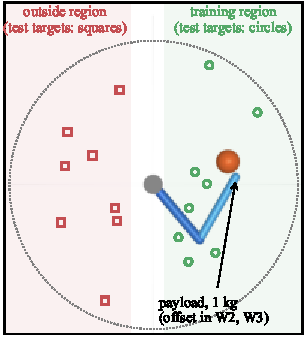
\includegraphics[width=0.9\columnwidth]{setup}
\caption{The arm with its payload, the region where training data was collected (right, $x \ge \SI{0.05}{m}$) and the region it never aimed at (left, $x \le \SI{-0.1}{m}$), with the targets of the 8 test tasks in each.}
\label{fig:setup}
\end{figure}

\subsection{Controller}

All methods share one sampling-based MPC with path-integral weighting \cite{williams2017model}.
Every \SI{20}{ms} it perturbs its current torque plan to form 256 candidates over a \SI{0.2}{s} horizon, predicts each candidate with the method's model, scores it by the squared tip-to-target distance plus a joint-speed penalty, and blends the candidates with weights that decrease exponentially with cost.
Only the first torque of the blended plan is applied.
The settings were tuned once, on development tasks, and then fixed for every method; only the predictor changes.

\subsection{Methods}

Table~\ref{tab:methods} lists the predictors.
The hand-written model of the arm, including the offset payload and friction terms needed by the reference, was checked against the simulator's inertia matrix and bias forces and reproduces the simulator step for step when given the true parameters.
\Co{} fits the payload mass by Gauss--Newton least squares on the one-period velocity prediction error.
The networks in \Ct{} and \Cr{} take the sines and cosines of the joint angles, the joint speeds and the torques, and predict the base model's error in angles and speeds after one \SI{20}{ms} period.
They have two hidden layers of 64 tanh units and are trained with Adam and early stopping on held-out episodes.
The ensembles add four networks that differ only in their random initialisation.

\begin{table}[t]
\centering
\caption{Methods. All use the same MPC; only the predictor differs.}
\label{tab:methods}
\footnotesize
\begin{tabular}{@{}lp{6.2cm}@{}}
\toprule
\Cz & physics model assuming no payload\\
\Co & physics model with the payload mass estimated from data\\
\Ct & \Cz's model plus a residual network\\
\Cr & \Co's model plus a residual network\\
\Ct-E, \Cr-E & as \Ct, \Cr, with the average of five networks; optionally the MPC is penalised for the networks' disagreement\\
Reference & physics model told the true payload and world (an upper bound, not a method)\\
\bottomrule
\end{tabular}
\end{table}

\subsection{Data and protocol}

Data is recorded by running \Cz{} with random torque perturbations towards random targets in the training region, in \SI{3}{s} episodes, and is measured in seconds of motion: budgets of 9, 30 and \SI{90}{s}, with smaller budgets being the first episodes of the largest.
Data is always split by whole episodes.

Every choice (MPC settings, network size and training, penalty weight) was made on development material only: a separate data seed, a separate validation set and separate development tasks.
The test material consists of three further data seeds and 8 reaching tasks inside and 8 outside the training region (Fig.~\ref{fig:setup}), giving 24 runs per method, world and budget.
A run lasts \SI{3}{s}; its final error is the mean tip error over the last \SI{0.5}{s}, and it counts as not settled if the error at the end exceeds \SI{1}{cm}.
Re-running the inside tasks in a later experiment reproduced all 792 earlier runs exactly.

\section{Results}

\subsection{Prediction}

Fig.~\ref{fig:prediction} shows how far each model's prediction of the tip drifts in \SI{0.2}{s}, the MPC's horizon.
\Co{} is exact in W1 with any amount of data, but in W2 and W3 it leaves an error of about 2.5--\SI{4}{cm} that more data does not reduce: it can only explain the offset payload and friction by overestimating the mass (about \SI{1.2}{kg}).
\Ct{} needs data: with \SI{9}{s} it is far worse than \Co{}, with \SI{90}{s} far better.
\Cr{} is the most accurate throughout, because its network only has to learn what \Co{} leaves.
Outside the training region the learned models degrade by roughly an order of magnitude, while \Co{} does not.

\begin{figure*}[t]
\centering
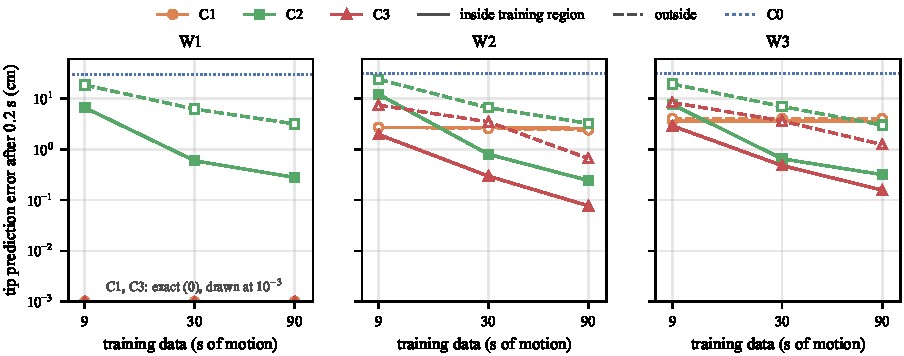
\includegraphics[width=\textwidth]{prediction}
\caption{Tip prediction error after \SI{0.2}{s} against the amount of training data (mean of three data seeds), on validation episodes inside (filled, solid) and outside (open, dashed) the training region. The reference model is exact everywhere.}
\label{fig:prediction}
\end{figure*}

\subsection{Control inside the training region}

Fig.~\ref{fig:control} (solid lines) and Table~\ref{tab:key} show control results.
\Cz{} stops 8--\SI{10}{cm} from the target.
\Co{} settles about \SI{2}{cm} away in W2 and W3, consistently, with almost no spread.
With \SI{30}{s} of data or more, the learned methods do better; with \SI{90}{s}, \Cr{} reaches \SI{0.07}{cm} in W2, close to the reference (\SI{0.04}{cm}).
With \SI{9}{s} the picture reverses: \Ct{} is worse than \Co{}, and in W2 one run ends \SI{68}{cm} from the target.
The two kinds of method fail differently: \Co{} is consistently a little off, the learned methods are usually precise but occasionally far off.

\begin{figure*}[t]
\centering
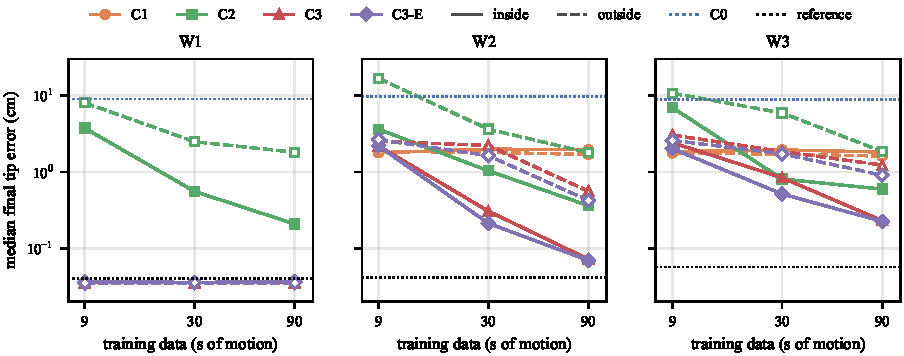
\includegraphics[width=\textwidth]{control}
\caption{Median final tip error over 24 runs (8 tasks, 3 data seeds) against the amount of training data, for test tasks inside (solid) and outside (dashed) the training region. Dotted lines: \Cz{} and the reference.}
\label{fig:control}
\end{figure*}

\begin{table}[t]
\centering
\caption{Median final tip error in cm (runs not settled, of 24). \Cr-E averages five networks without penalty.}
\label{tab:key}
\footnotesize
\setlength{\tabcolsep}{3pt}
\begin{tabular}{llrccccc}
\toprule
Tasks & World & Data & C1 & C2 & C3 & C3-E & Ref.\\
\midrule
inside & W2 & 30\,s & 1.99 (24) & 1.03 (11) & 0.31 (4) & 0.21 (2) & 0.04 (0)\\
inside & W2 & 90\,s & 1.95 (22) & 0.36 (4) & 0.07 (1) & 0.07 (0) & 0.04 (0)\\
inside & W3 & 30\,s & 1.94 (24) & 0.81 (9) & 0.84 (8) & 0.51 (6) & 0.06 (0)\\
inside & W3 & 90\,s & 1.82 (22) & 0.59 (6) & 0.23 (4) & 0.23 (3) & 0.06 (0)\\
\midrule
outside & W2 & 30\,s & 1.79 (20) & 3.63 (22) & 2.22 (21) & 1.63 (17) & 0.04 (0)\\
outside & W2 & 90\,s & 1.69 (19) & 1.78 (18) & 0.56 (6) & 0.42 (2) & 0.04 (0)\\
outside & W3 & 30\,s & 1.70 (18) & 5.91 (24) & 1.84 (18) & 1.73 (20) & 0.06 (0)\\
outside & W3 & 90\,s & 1.61 (17) & 1.85 (21) & 1.23 (15) & 0.90 (10) & 0.06 (0)\\
\bottomrule
\end{tabular}

\end{table}

\subsection{Control outside the training region}

Outside the training region (dashed lines in Fig.~\ref{fig:control}), \Co{} performs as it does inside, but the learned methods lose most of their advantage.
In W2 with \SI{90}{s} of data, \Ct{} goes from \SI{0.36}{cm} inside to \SI{1.78}{cm} outside, no better than \Co{}; with \SI{30}{s} it is twice as bad as \Co{}.
\Cr{} holds up better, staying ahead of \Co{} with \SI{90}{s} (\SI{0.56}{cm} against \SI{1.69}{cm}) but falling behind it with \SI{30}{s}.
Fig.~\ref{fig:worst} shows the three worst runs: on tasks that \Co{} solves directly, \Ct{} swings the arm through large loops and ends 49--\SI{66}{cm} away.

\begin{figure*}[t]
\centering
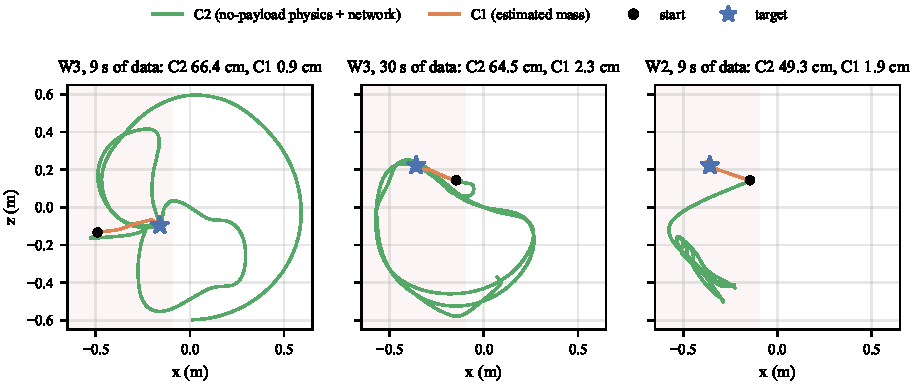
\includegraphics[width=\textwidth]{worst}
\caption{Tip paths of the three worst \Ct{} runs outside the training region (shaded), next to \Co{} on the same task, data seed and MPC seed.}
\label{fig:worst}
\end{figure*}

\subsection{Why: the controller's expectations are optimistic}

Every control round, the MPC predicts where the tip will be one period later under the torque it applies.
Comparing that prediction with where the tip actually goes measures the model's error along the path the controller chose.
For the learned models it grows 8--13 times outside the training region (\Ct{}, W2, \SI{30}{s}: from 0.0095 to \SI{0.079}{cm} per period), while for \Co{} it stays at \SI{0.03}{cm}.

The error is not random in direction.
We define optimism as how much closer to the target the model expected the tip to be than it actually was.
Random errors would average out near zero; instead, for every wrong model, physical or learned, inside or outside, optimism amounts to half to all of the prediction error (Fig.~\ref{fig:optimism}).
This is a selection effect: by picking the action its model rates best, the MPC systematically picks actions whose outcome the model overestimates.
What sets the learned models apart outside their data is not this mechanism but the size of the errors it acts on.

\begin{figure}[t]
\centering
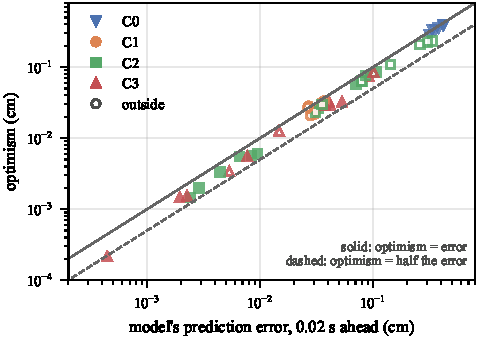
\includegraphics[width=\columnwidth]{optimism}
\caption{Median optimism against median one-period prediction error along the executed path, one point per method, world, data budget and task region (exact models omitted). All points lie between half and all of the error.}
\label{fig:optimism}
\end{figure}

\subsection{Ensembles}

Averaging five networks helps mostly with the tails (Fig.~\ref{fig:ensemble}, Table~\ref{tab:key}).
Outside the training region in W2 with \SI{90}{s} of data, the number of unsettled runs of physics plus learning drops from 6 to 2; with \SI{30}{s}, \Cr-E (\SI{1.63}{cm}) is no longer worse than \Co{} (\SI{1.79}{cm}), unlike the single-network \Cr{}.
With \SI{9}{s} of data, the ensemble does not help: all five networks are poor, and \Ct-E remains far worse than \Co{} outside the training region.

Penalising disagreement between the networks was meant to keep the MPC away from states the data did not cover.
On development tasks, penalty weights from 0.3 to 3000 changed the error by little, and on test tasks the penalised ensembles were neither consistently better nor worse than plain averaging.
A likely reason is that disagreement was measured one step ahead from the averaged state, where it is small, whereas errors build up over the horizon; propagating each network separately, as in \cite{chua2018deep}, would capture this at a higher cost.

Cost is the other limit.
Planning one round took about \SI{6}{ms} for \Co{}, \SI{11}{ms} for \Cr{} and \SI{28}{ms} for \Cr-E on the laptop CPU used, so the ensemble exceeds the \SI{20}{ms} control period.
The simulation waits for the controller, so this does not affect the results above, but the ensemble controller could not run in real time as implemented.

\begin{figure}[t]
\centering
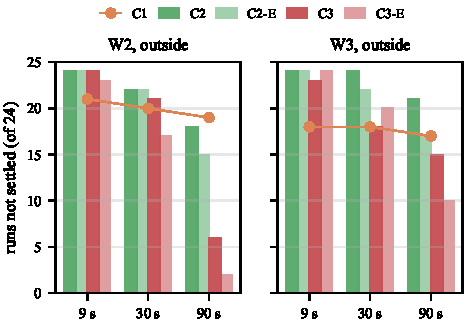
\includegraphics[width=\columnwidth]{ensemble}
\caption{Runs not settled (of 24) outside the training region: single networks (dark) against five-network averages (light), with \Co{} for reference.}
\label{fig:ensemble}
\end{figure}

\section{Discussion and Limitations}

Read practically, the results suggest: with little data, estimate the physical parameter; with more, add a learned residual on top of the physics and average several networks; and judge a learned controller by its worst runs and by where it will be used, not only by its median error inside the data it was trained on.

The study is deliberately narrow.
It is simulation only, with a planar two-link arm and one payload mass; ``outside'' is one region of the workspace; the ensemble members differ only in initialisation; and the model mismatches in W2 and W3 were chosen by hand to be large enough to matter.
The disagreement penalty was a simple one-step version and should not be read as evidence against uncertainty-aware planning in general.

\section{Conclusion}

In a controlled setting where every source of model error is known, a learned correction made a sampling-based MPC markedly more accurate when enough data was available and the task stayed where the data was collected, and markedly less reliable when either condition failed.
The mechanism is that the controller exploits whatever errors its model has, and learned models outside their data have large ones.
Physics plus an averaged ensemble was the most robust combination we tested, at a computational cost that needs to be addressed before it can run in real time.

\bibliographystyle{IEEEtran}
\bibliography{references}

\end{document}
